% **************************************************************************************************
% ** SPSC Report and Thesis Template
% **************************************************************************************************
%
% ***** Authors *****
% Daniel Arnitz, Paul Meissner, Stefan Petrik
% Signal Processing and Speech Communication Laboratory (SPSC)
% Graz University of Technology (TU Graz), Austria
%
% ***** Changelog *****
% 0.1   2010-01-25   extracted from report template by Daniel Arnitz (not ready yet)
% 0.2   2010-02-08   added thesis titlepage and modified layout (not ready yet)
% 0.3   2010-02-18   added TUG logo and statutory declaration
% 0.4   2010-02-18   moved the information fields below % **************************************************************************************************
% ** SPSC Report and Thesis Template
% **************************************************************************************************
%
% ***** Authors *****
% Daniel Arnitz, Paul Meissner, Stefan Petrik
% Signal Processing and Speech Communication Laboratory (SPSC)
% Graz University of Technology (TU Graz), Austria
%
% ***** Changelog *****
%
% ***** Todo *****
%
% **************************************************************************************************



\documentclass[%
a4paper,% !!! ATTENTION: geometry package below !!!
\Twosided,% !!! ATTENTION: geometry package below !!!
openany,% begin chapters with new right page (openright) or don't care (openany)
11pt,%
fleqn,% equations not centered, but on the left side
tablecaptionbelow,% captions below tables
% titlepage,% use title
pointlessnumbers,% do not generate point at the end of section numbers (e.g. 1.4.5 instead of 1.4.5.)
final,%
]{scrreprt}% (KOMA)

\usepackage[paper=a4paper,\Twosided,%
textheight=246mm,%
textwidth=160mm,%
heightrounded=true,% round textheight to multiple of lines (avoids overfull vboxes)
ignoreall=true,% do not include header, footer, and margins in calculations
marginparsep=5pt,% marginpar only used for signs (centered), thus only small sep. needed
marginparwidth=10mm,% prevent margin notes to be out of page
hmarginratio=2:1,% set margin ration (inner:outer for twoside) - (2:3 is default)
]{geometry}%


% master
\usepackage{ifthen}% for optional parts
\usepackage[latin1]{inputenc}% German special characters
\ifthenelse{\equal{\DocumentLanguage}{en}}{\usepackage[USenglish]{babel}}{}%
\ifthenelse{\equal{\DocumentLanguage}{de}}{\usepackage[ngerman]{babel}}{}%
\usepackage[%
headtopline,plainheadtopline,% activate all lines (header and footer)
headsepline,plainheadsepline,%
footsepline,plainfootsepline,%
footbotline,plainfootbotline,%
automark% auto update \..mark
]{scrpage2}% (KOMA)
\usepackage{makeidx}% used to make an index directory
\usepackage[]{caption}% customize captions
\usepackage{multicol}%
\usepackage[stable,bottom,hang,splitrule,multiple,symbol*]{footmisc}% customize footnotes


% text
\usepackage{varioref}% improved references
\usepackage{color}% e.g., for color boxes
\usepackage{rotating}% to rotate objects
\usepackage{gensymb}% symbols (perthousand, Celsius, ...)
\usepackage[right]{eurosym}% euro symbol on the right side (51 EUR)
\usepackage[normalem]{ulem}% cross-out, strike-out, underlines (normalem: keep \emph italic)
%\usepackage[safe]{textcomp}% loading in safe mode to avoid problems (see LaTeX companion)
%\usepackage[geometry,misc]{ifsym}% technical symbols
\usepackage{remreset}%\@removefromreset commands (e.g., for continuous footnote numbering)
\usepackage[%
breaklinks=true,% allow line break in links
colorlinks=true,% if false: framed link
linkcolor=black,anchorcolor=black,citecolor=black,filecolor=black,%
menucolor=black,urlcolor=black]{hyperref}% hyperlinks for references


% math
\usepackage{amsmath,amssymb,amstext,bm} % use math packages
\usepackage{mathcomp}% symbols (perthousand, ...) in math mode


% graphics
\usepackage{graphicx}% use simple graphics
\usepackage{subfigure}% subfigures (a),(b),(c)... within figures
\usepackage{flafter}% place floats always after reference
\usepackage{placeins}% preventing floats from crossing a barrier
\usepackage{float}% to place floats !HERE!
\usepackage{psfrag}% replace text in eps figures


% tables
\usepackage{hhline}% hline doesn't work with colored columns, so using hhline
\usepackage{longtable}% for tables longer than one page
\usepackage{dcolumn}% for number alignment in tables
\usepackage{colortbl}% color in tables


% listings
%\usepackage{alltt}% verbatim environment with commands available
\usepackage{listings}% program code listings


% other
%\usepackage{layout}% graphical page layout (spacings)
\usepackage{xspace}% add space after macros if not followed by punctuation character
\makeindex% used for index creation

 (encoding...)
% 0.5   2010-03-02   added \ShortTitle to fix problems with long thesis titles
%                    added \ThesisType (makes the template suitable for MSc, BSc, PhD, ... Thesis)
%
% ***** Todo *****
% - Introduction/Usage
% **************************************************************************************************

% **************************************************************************************************
% basic setup
\newcommand{\DocumentType}{report} % "thesis" / "report"
\newcommand{\DocumentLanguage}{de} % "en" / "de"
\newcommand{\Twosided}{} % "twoside" / ""


% **************************************************************************************************
% template setup -- do not change these unless you know what you are doing!
% **************************************************************************************************
% ** SPSC Report and Thesis Template
% **************************************************************************************************
%
% ***** Authors *****
% Daniel Arnitz, Paul Meissner, Stefan Petrik
% Signal Processing and Speech Communication Laboratory (SPSC)
% Graz University of Technology (TU Graz), Austria
%
% ***** Changelog *****
%
% ***** Todo *****
%
% **************************************************************************************************



\documentclass[%
a4paper,% !!! ATTENTION: geometry package below !!!
\Twosided,% !!! ATTENTION: geometry package below !!!
openany,% begin chapters with new right page (openright) or don't care (openany)
11pt,%
fleqn,% equations not centered, but on the left side
tablecaptionbelow,% captions below tables
% titlepage,% use title
pointlessnumbers,% do not generate point at the end of section numbers (e.g. 1.4.5 instead of 1.4.5.)
final,%
]{scrreprt}% (KOMA)

\usepackage[paper=a4paper,\Twosided,%
textheight=246mm,%
textwidth=160mm,%
heightrounded=true,% round textheight to multiple of lines (avoids overfull vboxes)
ignoreall=true,% do not include header, footer, and margins in calculations
marginparsep=5pt,% marginpar only used for signs (centered), thus only small sep. needed
marginparwidth=10mm,% prevent margin notes to be out of page
hmarginratio=2:1,% set margin ration (inner:outer for twoside) - (2:3 is default)
]{geometry}%


% master
\usepackage{ifthen}% for optional parts
\usepackage[latin1]{inputenc}% German special characters
\ifthenelse{\equal{\DocumentLanguage}{en}}{\usepackage[USenglish]{babel}}{}%
\ifthenelse{\equal{\DocumentLanguage}{de}}{\usepackage[ngerman]{babel}}{}%
\usepackage[%
headtopline,plainheadtopline,% activate all lines (header and footer)
headsepline,plainheadsepline,%
footsepline,plainfootsepline,%
footbotline,plainfootbotline,%
automark% auto update \..mark
]{scrpage2}% (KOMA)
\usepackage{makeidx}% used to make an index directory
\usepackage[]{caption}% customize captions
\usepackage{multicol}%
\usepackage[stable,bottom,hang,splitrule,multiple,symbol*]{footmisc}% customize footnotes


% text
\usepackage{varioref}% improved references
\usepackage{color}% e.g., for color boxes
\usepackage{rotating}% to rotate objects
\usepackage{gensymb}% symbols (perthousand, Celsius, ...)
\usepackage[right]{eurosym}% euro symbol on the right side (51 EUR)
\usepackage[normalem]{ulem}% cross-out, strike-out, underlines (normalem: keep \emph italic)
%\usepackage[safe]{textcomp}% loading in safe mode to avoid problems (see LaTeX companion)
%\usepackage[geometry,misc]{ifsym}% technical symbols
\usepackage{remreset}%\@removefromreset commands (e.g., for continuous footnote numbering)
\usepackage[%
breaklinks=true,% allow line break in links
colorlinks=true,% if false: framed link
linkcolor=black,anchorcolor=black,citecolor=black,filecolor=black,%
menucolor=black,urlcolor=black]{hyperref}% hyperlinks for references


% math
\usepackage{amsmath,amssymb,amstext,bm} % use math packages
\usepackage{mathcomp}% symbols (perthousand, ...) in math mode


% graphics
\usepackage{graphicx}% use simple graphics
\usepackage{subfigure}% subfigures (a),(b),(c)... within figures
\usepackage{flafter}% place floats always after reference
\usepackage{placeins}% preventing floats from crossing a barrier
\usepackage{float}% to place floats !HERE!
\usepackage{psfrag}% replace text in eps figures


% tables
\usepackage{hhline}% hline doesn't work with colored columns, so using hhline
\usepackage{longtable}% for tables longer than one page
\usepackage{dcolumn}% for number alignment in tables
\usepackage{colortbl}% color in tables


% listings
%\usepackage{alltt}% verbatim environment with commands available
\usepackage{listings}% program code listings


% other
%\usepackage{layout}% graphical page layout (spacings)
\usepackage{xspace}% add space after macros if not followed by punctuation character
\makeindex% used for index creation


\input{./base/layout_\DocumentType}
% **************************************************************************************************
% ** SPSC Report and Thesis Template
% **************************************************************************************************
%
% ***** Authors *****
% Daniel Arnitz, Paul Meissner, Stefan Petrik
% Signal Processing and Speech Communication Laboratory (SPSC)
% Graz University of Technology (TU Graz), Austria
%
% ***** Changelog *****
%
% ***** Todo *****
%
% **************************************************************************************************



% **************************************************************************************************
% * SECTIONING AND TEXT
% **************************************************************************************************

% new chapter, section, ... plus a few addons
%   part
\newcommand{\newpart}[2]{\FloatBarrier\cleardoublepage\part{#1}\label{part:#2}}%
%   chapter
\newcommand{\newchapter}[2]{\FloatBarrier\chapter{#1}\label{chp:#2}}
\newcommand{\newchapterNoTOC}[2]{\FloatBarrier\stepcounter{chapter}\chapter*{#1}\label{chp:#2}}%
%   section
\newcommand{\newsection}[2]{\FloatBarrier\vspace{5mm}\section{#1}\label{sec:#2}}%
\newcommand{\newsectionNoTOC}[2]{\FloatBarrier\vspace{5mm}\stepcounter{section}\section*{#1}\label{sec:#2}}%
%   subsection
\newcommand{\newsubsection}[2]{\FloatBarrier\vspace{3mm}\subsection{#1}\label{sec:#2}}%
\newcommand{\newsubsectionNoTOC}[2]{\FloatBarrier\vspace{3mm}\stepcounter{subsection}\subsection*{#1}\label{sec:#2}}%
%   subsubsection
\newcommand{\newsubsubsection}[2]{\vspace{2mm}\subsubsection{#1}\label{sec:#2}}%
\newcommand{\newsubsubsectionNoTOC}[2]{\vspace{2mm}\stepcounter{subsubsection}\subsubsection*{#1}\label{sec:#2}}%

% next paragraph
\newcommand{\nxtpar}{\par\bigskip}

% "stylish" quotes on the right side
\newcommand{\openingquote}[2]{\hfill\parbox[t]{10cm}{\itshape\raggedleft{"#1"}\\\footnotesize -- #2}\nxtpar}%

% direct quotes
% \newenvironment{directquote}{\nxtpar\hrule}{\hrule}\hfill\litref{#1}{#2}}

% warnings and attention signs in marginpar
\newcommand{\MDanger}{\marginpar{\Huge\centering\fbox{\textbf{!}}}}%
\newcommand{\MAttention}{\marginpar{\Huge\centering\textbf{!}}}%
\newcommand{\MHint}{\marginpar{\Huge\centering\textbf{\checkmark}}}%
\newcommand{\MQuestion}{\marginpar{\Huge\centering\textbf{?}}}%

% same footnote number as last one
\newcommand{\lastfootnotemark}{\addtocounter{footnote}{-1}\footnotemark}%

% value-unit commands (for 457 kHz, etc)
\newcommand{\vu}[2]{\mbox{$#1\,\text{#2}$}} % "value~unit" ... prevents e.g. 456 \linebreak mV
\newcommand{\vuc}[3]{\mbox{$#1\,\text{#2}\;#3\,\%$}} % "value~unit~tolerance-per-cent"
\newcommand{\vum}[3]{\mbox{$#1\,\text{#2}\;#3\,\perthousand$}} % "value~unit~tolerance-per-mil"

% reminders
\newcommand{\reminder}[1]{\colorbox{red}{#1}\xspace}%
\newcommand{\rem}{\reminder{(...)}}%
\newcommand{\remq}{\reminder{???}}%
\newcommand{\uc}{\nxtpar\colorbox{yellow}{... under construction ...}\nxtpar}%

% misc
\newcommand{\pwd}{.} % present working directory (can be used to create relativ paths per part, etc.)


% **************************************************************************************************
% * MATH
% **************************************************************************************************

% highlighting
\newcommand{\vm}[1]{\bm{#1}}% vector or matrix

% operators
\newcommand{\E}[1]{\text{E}\!\left\{#1\right\}}% expectation operator
\newcommand{\var}[1]{\text{var}\!\left\{#1\right\}}% variance operator
\renewcommand{\ln}[1]{\text{ln}\!\left(#1\right)}% natural logarithm
\newcommand{\ld}[1]{\text{ld}\!\left(#1\right)}% logarithm base 2
\renewcommand{\log}[1]{\text{log}\!\left(#1\right)}% logarithm (base 10)
\newcommand{\logb}[2]{\text{log}_{#1}\!\left(#2\right)}% logarithm base ...
\newcommand{\avgvar}[1]{\overline{\text{var}}\!\left\{#1\right\}}% average variance operator
\renewcommand{\Re}[1]{\text{Re}\!\left\{#1\right\}}% real part
\renewcommand{\Im}[1]{\text{Im}\!\left\{#1\right\}}% imaginary part

% other
\newcommand{\conj}{^\ast}% conjugate complex
\newcommand{\mtx}[2]{\left[\begin{array}{#1}#2\end{array}\right]}%vector/matrix


% **************************************************************************************************
% * FLOATS (FIGURES, TABLES, LISTINGS, ...)
% **************************************************************************************************

% figures without frames
%   standard
\newcommand{\fig}[3]{\begin{figure}\centering\includegraphics[width=\textwidth]{#1}\caption{#2}\label{fig:#3}\end{figure}}%
%   with controllable parameters
\newcommand{\figc}[4]{\begin{figure}\centering\includegraphics[#1]{#2}\caption{#3}\label{fig:#4}\end{figure}}%
%   two subfigures
\newcommand{\twofig}[6]{\begin{figure}\centering%
\subfigure[#2]{\includegraphics[width=0.495\textwidth]{#1}}%
\subfigure[#4]{\includegraphics[width=0.495\textwidth]{#3}}%
\caption{#5}\label{fig:#6}\end{figure}}%
%   two subfigures and controllable parameters
\newcommand{\twofigc}[8]{\begin{figure}\centering%
\subfigure[#3]{\includegraphics[#1]{#2}}%
\subfigure[#6]{\includegraphics[#4]{#5}}%
\caption{#7}\label{fig:#8}\end{figure}}%

% framed figures
%   standard
\newcommand{\figf}[3]{\begin{figure}\centering\fbox{\includegraphics[width=\textwidth]{#1}}\caption{#2}\label{fig:#3}\end{figure}}%
%   with controllable parameters
\newcommand{\figcf}[4]{\begin{figure}\centering\fbox{\includegraphics[#1]{#2}}\caption{#3}\label{fig:#4}\end{figure}}%
%   two subfigures
\newcommand{\twofigf}[6]{\begin{figure}\centering%
\fbox{\subfigure[#2]{\includegraphics[width=0.495\textwidth]{#1}}}%
\fbox{\subfigure[#4]{\includegraphics[width=0.495\textwidth]{#3}}}%
\caption{#5}\label{fig:#6}\end{figure}}%
%   two subfigures and controllable parameters
\newcommand{\twofigcf}[8]{\begin{figure}\centering%
\fbox{\subfigure[#3]{\includegraphics[#1]{#2}}}%
\fbox{\subfigure[#6]{\includegraphics[#4]{#5}}}%
\caption{#7}\label{fig:#8}\end{figure}}%

% listings
\newcommand{\filelisting}[4]{\lstinputlisting[print=true,language=#1,caption={#3},label={lst:#4}]{#2}}

% preserve backslash for linebreaks in tables (ragged... redefines \\, thus it has to be preserved)
\newcommand{\pbs}[1]{\let\temp=\\#1\let\\=\temp}%

\graphicspath{{./drawings/}{./plots/}{./images/}}
% **************************************************************************************************
% ATTENTION: Make sure that makeindex is set to -s "./base/index.sty"
% **************************************************************************************************

% uncomment to get watermarks:
% \usepackage[first,bottom,light,draft]{draftcopy}
% \draftcopyName{ENTWURF}{160}


% **************************************************************************************************
% information fields

% general
\newcommand{\DocumentTitle}{Adaptive Systems}
\newcommand{\DocumentSubtitle}{Assignment 3}
\newcommand{\ShortTitle}{Assignment 3} % used in headers (keep short!)
\newcommand{\DocumentAuthor}{Ebner Thomas (0831246), N�hmer Stefan (0830668)}
\newcommand{\DocumentDate}{Graz, \today}
%    for thesis only (will be ignored for reports)
\newcommand{\ThesisType}{Master's Thesis}
\newcommand{\Organizations}{Signal Processing and Speech Communications Laboratory \\ Graz University of Technology \\[1cm] on behalf of \\ Some Company} % SPSC \\ TUG \\[1cm] on behalf of \\ A Nice Company
\newcommand{\Advisors}{Dipl.-Ing. Dr. Assoc.Prof. Klaus Witrisal \\ Dipl.-Ing. Paul Meissner} % Advisor 1 \\ Advisor 2 \\ ...
\newcommand{\Supervisors}{Univ.-Prof. Dipl.-Ing. Dr.techn. Gernot Kubin}

% revision number
\newcommand{\RevPrefix}{alpha~}
\newcommand{\RevLarge}{1}
\newcommand{\RevSmall}{0}

% confidential?
\newcommand{\ConfidNote}{do not blend}% {"confidential", "eyes only", ...}





\begin{document}

%listingstyle:
\definecolor{orange}{rgb}{0.75,0.65,0}
\definecolor{gruen}{rgb}{0,0.5,0}
\definecolor{listinggray}{gray}{0.97}
\definecolor{listingshadow}{gray}{0.2}
\lstloadlanguages{Matlab}
\lstset{frame=shadowbox,
		rulesepcolor=\color{listingshadow},
		numbers=left,
		basicstyle=\scriptsize\ttfamily,
		numberstyle=\tiny,
		keywordstyle=\color{blue}\bfseries, % bold black keywords
		identifierstyle=, % nothing happens
		commentstyle=\color{gruen}, % comments
		stringstyle=\color{orange}, % typewriter type for strings
		showstringspaces=false,
		tabsize=4,
		backgroundcolor=\color{listinggray}
        }




% **************************************************************************************************
% titlepage
\input{./base/titlepage_\DocumentType}

% statutory declaration for theses
\ifthenelse{\equal{\DocumentType}{thesis}}{% **************************************************************************************************
% ** SPSC Report and Thesis Template
% **************************************************************************************************
%
% ***** Authors *****
% Daniel Arnitz, Paul Meissner, Andreas Laesser, Stefan Petrik
% Signal Processing and Speech Communication Laboratory (SPSC)
% Graz University of Technology (TU Graz), Austria
%
% ***** Changelog *****
% 0.1   2010-02-18   created
% 0.2   2010-03-02   added German declaration
%
% ***** Todo *****
% **************************************************************************************************

\cleardoublepage
\pagestyle{empty}\pagenumbering{roman}

\vspace*{1cm}

% English
\ifthenelse{\equal{\DocumentLanguage}{en}}{
\begin{center}\Large\bfseries Statutory Declaration\end{center}\vspace*{1cm}
\noindent I declare that I have authored this thesis independently, that I have not used other than the declared sources$/$resources, and that I have explicitly marked all material which has been quoted either literally or by content from the used sources.
\par\vspace*{4cm}
\centerline{
\begin{tabular}{m{1.5cm}cm{1.5cm}m{3cm}m{1.5cm}cm{1.5cm}}
\cline{1-3} \cline{5-7}
 & date & & & & (signature) &\\
\end{tabular}}
}

% German
\ifthenelse{\equal{\DocumentLanguage}{de}}{
\begin{center}\Large\bfseries Eidesstattliche Erkl�rung\end{center}\vspace*{1cm}
Ich erkl�re an Eides statt, dass ich die vorliegende Arbeit selbstst�ndig verfasst, andere als die angegebenen Quellen$/$Hilfsmittel nicht benutzt, und die den benutzten Quellen w�rtlich und inhaltlich entnommene Stellen als solche kenntlich gemacht habe.
\par\vspace*{4cm}
\centerline{
\begin{tabular}{m{1.5cm}cm{1.5cm}m{3cm}m{1.5cm}cm{1.5cm}}
\cline{1-3} \cline{5-7}
 & Graz, am & & & & (Unterschrift) &\\
\end{tabular}}
}

}{}


% **************************************************************************************************
% **************************************************************************************************
% user-defined part

\chapter{Analytical Problem 3.1: Predictive Encoding of an AR Process}

\paragraph{a)}


\clearpage
\chapter{Matlab Problem 3.2: Information vs. Energy}

Zur Berechnung der Ausgangswerte des Systems wurde das System mit dem vorgegebenen Quantizer implementiert (siehe Listings) und f�r $10^6$ Samples mit 1 bis 5 Bit Simulationen durchgef�hrt. Der Quantisierer f�hrt teilt dabei den Eingangsbereich in eine der Anzahl an Bit entsprechenden Anzahl Stufen und rundet das Eingangssignal auf die n�chstliegende Stufe.

Mit der vorgegebenen Funktion \texttt{CondEntropy} wurden die bedingten Entropien berechnet, welche dem Informationsgehalt eines Wertes entspricht, wenn die vorherigen Werte bekannt sind.

Darstellungen \ref{fig:3_2_h_N0}, \ref{fig:3_2_h_N1} und \ref{fig:3_2_h_N2} stellen die bedingten Entropien bei unterschiedlichen $N$ dar.

Bei $N=0$ (Abb.~\ref{fig:3_2_h_N0}) sinkt die Entropie nach dem ersten Zeichen schnell, und danach langsamer. F�hrt man \emph{Linear Prediction} ein mit $N=1$ (Abb.~\ref{fig:3_2_h_N1}), so bleibt die Entropie weitgehend erhalten und sinkt nur langsam, der Informationsgehalt der �bertragenen Werte bleibt also h�her. Erh�ht man $N$ auf $2$ (Abb.~\ref{fig:3_2_h_N2}), so beginnt die Entropie wieder zu sinken, und zwar sogar schneller als im Fall $N=0$.

\begin{figure}[h!]
  \centering
  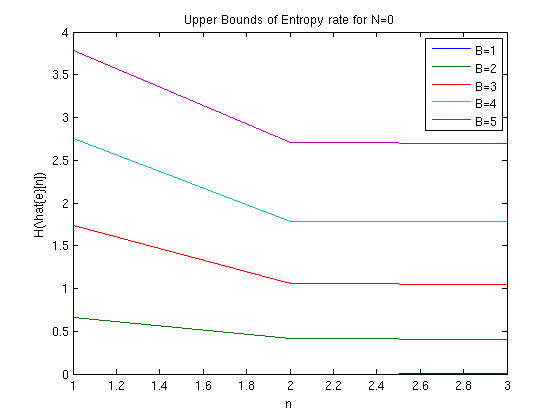
\includegraphics[width=0.7\textwidth]{./plots/3_2_h_N0.png}
  % 3_3_c_freqresponse.png: 560x420 pixel, 90dpi, 15.81x11.85 cm, bb=0 0 448 336
  \caption{Entropie f�r $N=0$}
  \label{fig:3_2_h_N0}
\end{figure}

\begin{figure}[h!]
  \centering
  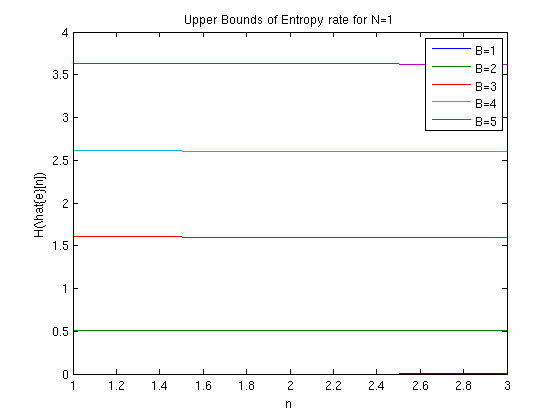
\includegraphics[width=0.7\textwidth]{./plots/3_2_h_N1.png}
  % 3_3_c_freqresponse.png: 560x420 pixel, 90dpi, 15.81x11.85 cm, bb=0 0 448 336
  \caption{Entropie f�r $N=1$}
  \label{fig:3_2_h_N1}
\end{figure}

\begin{figure}[h!]
  \centering
  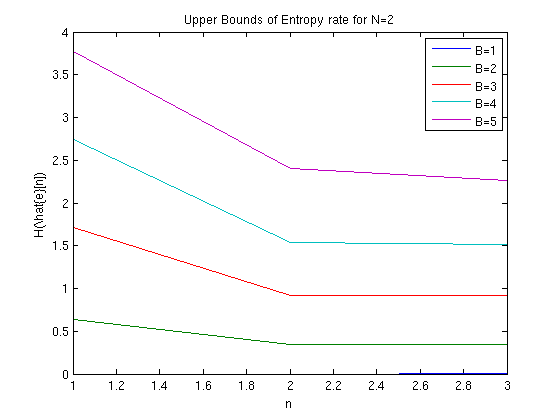
\includegraphics[width=0.7\textwidth]{./plots/3_2_h_N2.png}
  % 3_3_c_freqresponse.png: 560x420 pixel, 90dpi, 15.81x11.85 cm, bb=0 0 448 336
  \caption{Entropie f�r $N=2$}
  \label{fig:3_2_h_N2}
\end{figure}

\clearpage
\chapter{Analytical Problem 3.3: Least Squares IIR Identification}

Wir kennen das IIR-System $u[n] = v[n] + u[n-1] - \frac{1}{8} u[n-2]$, von dem $M$ Input-Output-Samples vorhanden sind.
F�r die folgende Differenzengleichung sollen die Parameter $a_k$ und $b_k$ bestimmt werden, wobei die Anzahl der Parameter $N = N_a + N_b + 1$ ist und $M \geq N$ ist:

\begin{equation}
  u[n] = \sum_{k=0}^{N_b} b_k v[n-k] - \sum_{k=1}^{N_a} a_k u[n-k]
\end{equation}


\paragraph{a)}

Es soll eine LS-L�sung (\emph{least squares}) f�r die Parameter gefunden werden.

Dazu wird zun�chst ein Parametervektor $\mathbf{c} = \begin{bmatrix} \mathbf{b} \\ - \mathbf{a} \end{bmatrix}$ eingef�hrt.

Weiters muss ein \emph{tap input/output vector} $\mathbf{x}[n] = \begin{bmatrix} \mathbf{v}[n] \\ \mathbf{u}[n] \end{bmatrix}$ eingef�hrt werden, mit $\mathbf{v}[n] = \begin{bmatrix} v[n-0] \\ v[n-1] \\ \vdots \\ v[n - N_b] \end{bmatrix}$ und $\mathbf{u}[n] = \begin{bmatrix} u[n-1] \\ u[n-2] \\ \vdots \\ u[n - N_a] \end{bmatrix}$.

F�r die LS-Solution gehen wir nun wie gewohnt vor. Der quadratische Fehler soll minimiert werden ($e[n]$ ist der Fehler, $d[n]$ das gew�nschte Signal). Dazu wird eine einfache Gleichung aufgestellt und in Vektorschreibweise �bergef�hrt:

\begin{equation}
  e[n] = d[n] - y[n] = d[n] - \mathbf{c}^T \mathbf{x}[n] = d[n] - \mathbf{x}^T[n] \mathbf{c} \;\; \Rightarrow \mathbf{e} = \mathbf{d} - \mathbf{X} \mathbf{c}
\end{equation}

$\mathbf{X}$ ist die Designmatrix mit folgender Struktur:

\begin{equation}
  \mathbf{X} = \begin{bmatrix} \mathbf{x}^T[0] \\ \mathbf{x}^T[1] \\ \vdots \\ \mathbf{x}^T[M] \end{bmatrix}
\end{equation}

Jetzt bestimmen wir die LS-Solution wie gehabt:

\begin{eqnarray}
  J(\mathbf{c}) & = & \sum_{n=0}^{M} \left| e[n] \right|^2 = \left| \left| \mathbf{e} \right| \right|^2 = \langle \mathbf{e}, \mathbf{e} \rangle = \mathbf{e}^T \mathbf{e} = (\mathbf{d} - \mathbf{X} \mathbf{c})^T (\mathbf{d} - \mathbf{X} \mathbf{c}) = (\mathbf{d}^T - \mathbf{c}^T \mathbf{X}^T) (\mathbf{d} - \mathbf{X} \mathbf{c}) \\
  & = & \mathbf{d}^T \mathbf{d} - \mathbf{d}^T \mathbf{X} \mathbf{c} - \underbrace{\mathbf{c}^T \mathbf{X}^T \mathbf{d}}_{\mathbf{d}^T \mathbf{X} \mathbf{c}} + \mathbf{c}^T \mathbf{X}^T \mathbf{X} \mathbf{c} = \mathbf{d}^T \mathbf{d} - 2 \mathbf{d}^T \mathbf{X} \mathbf{c} + \mathbf{c}^T \mathbf{X}^T \mathbf{X} \mathbf{c}
\end{eqnarray}

Die L�sung ergibt sich durch Ableiten und Null setzen der Kostenfunktion:

\begin{eqnarray}
  \mathbf{\triangledown}_{\mathbf{c}} J(\mathbf{c}) & = & 0 - 2 \mathbf{d}^T \mathbf{X} + 2 \mathbf{c}^T \mathbf{X}^T \mathbf{X} \stackrel{!}{=} 0 \\
  & \Rightarrow & \mathbf{d}^T \mathbf{X} \stackrel{!}{=} \mathbf{c}^T \mathbf{X}^T \mathbf{X} \\
  & \Rightarrow & \mathbf{X}^T \mathbf{d} \stackrel{!}{=} \mathbf{X}^T \mathbf{X}^T \mathbf{c} \\
  & & \Rightarrow \mathbf{c}_{LS} = (\mathbf{X}^T \mathbf{X})^{-1} \mathbf{X}^T \mathbf{d}
\end{eqnarray}

Aus dieser L�sung kann man die Parameter $\{ a_k \}$ und $\{b_k\}$ ablesen (siehe oben).

Diese L�sung entspricht der LS-Solution f�r FIR-Filter! $\mathbf{X}$ und $\mathbf{d}$ haben jedoch wie oben beschrieben eine spezielle Form \footnote{f�r die nicht vorhandenen Werte (z.B. $v[-1]$) wird 0 eingesetzt.}:

\begin{equation}
  \mathbf{X} = \begin{bmatrix} \mathbf{x}^T[0] \\ \mathbf{x}^T[1] \\ \vdots \\ \mathbf{x}^T[M] \end{bmatrix}
  = \begin{bmatrix} v[0] & v[-1] & v[-2] & \cdots & v[-N_b] & u[-1] & u[-2] & \cdots & u[-N_a] \\
                    v[1] & v[0] & v[-1] & \cdots & v[-(N_b+1)] & u[0] & u[-1] & \cdots & u[-(N_a+1)] \\
                    v[2] & v[1] & v[0] & \cdots & v[-(N_b+2)] & u[1] & u[0] & \cdots & u[-(N_a+2)] \\
                    \vdots & \ddots \end{bmatrix}
\end{equation}

Das gew�nschte Signal $d[n]$ entspricht dem Ausgangssignal des IIR-Filters:

\begin{equation}
  d[n] = v[n] + d[n-1] - \frac{1}{8} d[n-2] \;\; \Rightarrow \mathbf{d} = \begin{bmatrix} v[0] + 0 - \frac{1}{8} 0 \\ v[1] + v[0] - \frac{1}{8} 0 \\ v[2] + (v[1] + v[0]) - \frac{1}{8} v[0] \\ v[3] + (v[2] + v[1] + v[0] - \frac{1}{8} v[0]) - \frac{1}{8} (v[1] + v[0]) \\ \vdots \end{bmatrix}
\end{equation}


\paragraph{b)}

Nun soll f�r die Eingangsfolge $\{v[n]\} = \{1, 0, 0\}$ die Ausgangsfolge $\{u[n]\}$ berechnet werden. F�r die Anzahl der Parameter gilt $N_a = 1, N_b = 0$, es gibt also nur 2 Parameter: $a_1$ und $b_0$.

Wir evaluieren nun die Differenzengleichung f�r ein paar Iterationen (die Werte werden sp�ter ben�tigt):

\begin{eqnarray}
  u[n] & = & v[n] + u[n-1] - \frac{1}{8} u[n-2] \\
  \Rightarrow u[0] & = & v[0] + u[-1] - \frac{1}{8} u[-2] = v[0] + 0 - \frac{1}{8} 0 = v[0] = 1 \\
  u[1] & = & v[1] + u[0] - \frac{1}{8} u[-1] = 1 \\
  u[2] & = & v[2] + u[1] - \frac{1}{8} u[0] = 0 + 1 - \frac{1}{8} 1 = \frac{7}{8} \\
  u[3] & = & v[3] + u[2] - \frac{1}{8} u[1] = 0 + \frac{7}{8} - \frac{1}{8} 1 = \frac{3}{4} \\
  u[4] & = & v[4] + u[3] - \frac{1}{8} u[2] = 0 + \frac{3}{4} - \frac{1}{8} \frac{7}{8} = \frac{41}{64} \\
  u[5] & = & v[5] + u[4] - \frac{1}{8} u[3] = 0 + \frac{41}{64} - \frac{1}{8} \frac{3}{4} = \frac{35}{64} \\
  \vdots
\end{eqnarray}

Mit diesen berechneten Werten kann man nun die Matrix $\mathbf{X}$ und den Vektor $\mathbf{d}$ aufstellen (f�r die vorher berechneten 5 Iterationen):

\begin{equation}
  \mathbf{X} = \begin{bmatrix} v[0] & u[-1] \\ v[1] & u[0] \\ v[2] & u[1] \\ v[3] & u[2] \\ v[4] & u[3] \\ v[5] & u[4] \end{bmatrix} = 
  \begin{bmatrix} 1 & 0 \\ 0 & 1 \\ 0 & 1 \\ 0 & \frac{7}{8} \\ 0 & \frac{3}{4} \\ 0 & \frac{41}{64} \end{bmatrix},
  \;\;\;
  \mathbf{d} = \begin{bmatrix} u[0] \\ u[1] \\ u[2] \\ u[3] \\ u[4] \\ u[5] \end{bmatrix} = 
  \begin{bmatrix} 1 \\ 1 \\ \frac{7}{8} \\ \frac{3}{4} \\ \frac{41}{64} \\ \frac{35}{64} \end{bmatrix}
\end{equation}

Mit der oben aufgestellten Formel f�r $\mathbf{c}_{LS}$ berechnen wir nun die Parameter $a_1$ und $b_0$ (in Matlab):

\begin{equation}
  \mathbf{c}_{LS} = (\mathbf{X}^T \mathbf{X})^{-1} \mathbf{X}^T \mathbf{d} \stackrel{Matlab}{=} \begin{bmatrix} 1 \\ 0.8993 \end{bmatrix} \; \Rightarrow b_0 = 1, a_1 = -0.8993
\end{equation}


\paragraph{c)}

Verglichen mit dem Modell aus Problem 3.1 mit N=1 stimmen die Parameter gut �berein. Im Problem 3.3 kommt es jedoch stark darauf an, wie viele Iterationen f�r die Berechnung von $\mathbf{c}_{LS}$ verwendet werden. Je mehr Iterationen, desto genauer wird das Ergebnis (desto genauer kommt es an das Ergebnis von Problem 3.1 heran). Das liegt in der Natur des IIR-Filters, da es sehr lange dauert, bis die Ausgangswerte des IIR-Filters auf vernachl�ssigbar kleine Werte gesunken sind.

Zur Bestimmung der Frequence response bringen wir die Differenzengleichung zuerst in den z-Bereich:

\begin{equation}
  u[n] = b_0 v[n] - a_1 u[n-1] \;\; \Leftrightarrow \;\; U(z) = b_0 V(z) - a_1 U(z) z^{-1}
\end{equation}

Nun stellen wir die �bertragungsfunktion $H(z)$ auf:

\begin{equation}
  H(z) = \frac{U(z)}{V(z)} = \frac{b_0}{1 + a_1 z^{-1}} = b_0 \frac{z}{z + a_1}
\end{equation}

Mit dem Befehl \texttt{freqz} kann man in Matlab die Frequency response dieses Systems plotten. Das Ergebnis ist in Abbildung~\ref{fig:3_3_c_freqresponse} dargestellt.

\begin{figure}[h!]
  \centering
  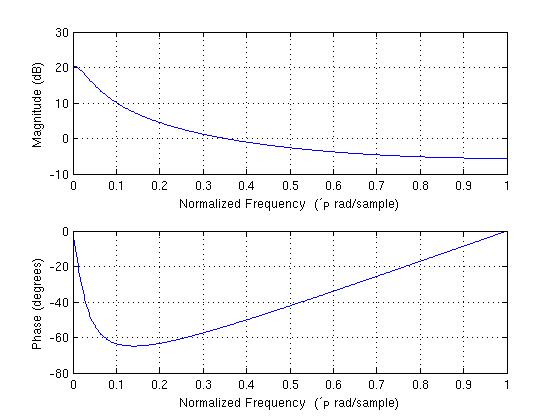
\includegraphics[width=0.7\textwidth]{./plots/3_3_c_freqresponse.png}
  % 3_3_c_freqresponse.png: 560x420 pixel, 90dpi, 15.81x11.85 cm, bb=0 0 448 336
  \caption{Frequency response des Systems aus Problem 3.3}
  \label{fig:3_3_c_freqresponse}
\end{figure}

\begin{figure}[h!]
  \centering
  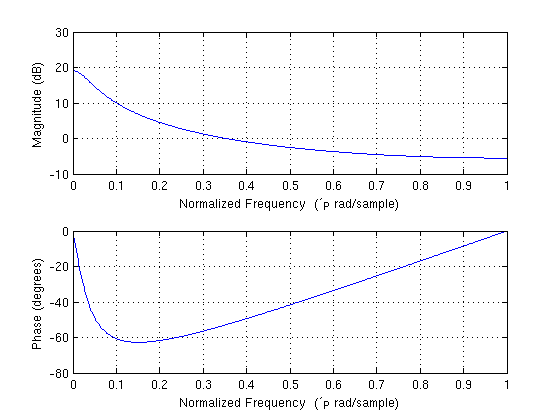
\includegraphics[width=0.7\textwidth]{./plots/3_1_d_freqresponse.png}
  % 3_3_c_freqresponse.png: 560x420 pixel, 90dpi, 15.81x11.85 cm, bb=0 0 448 336
  \caption{Frequency response des Systems aus Problem 3.1}
  \label{fig:3_1_d_freqresponse}
\end{figure}

\begin{LARGE}TODO\end{LARGE} Die Frequency response stimmt gut mit der von Problem 3.1 �berein. Man erkennt die �hnlichkeit der beiden Probleme.

Bei der R�cktransformation der �bertragungsfunktion aus dem z-Bereich ergibt sich f�r die Impulsantwort (mit Hilfe einer Transformationstabelle):

\begin{equation}
  h[n] = b_0 \cdot (-a_1)^n
\end{equation}

Daraus kann der Noise Gain berechnet werden:

\begin{equation}
  NG = \left|\left| \mathbf{h} \right| \right|^2 = \sum_{n=0}^{\infty} (b_0 (-a_1)^n)^2 = b_0^2 \sum_{n=0}^{\infty} (-a_1)^{2n} = 1^2 \sum_{n=0}^{\infty} (0.8993)^{2n} = \sum_{n=0}^{\infty} (0.8993^2)^n = \frac{1}{1 - 0.8993^2} = 5.23
\end{equation}

Dieser ist auch wieder h�her als bei Problem 3.1, nimmt aber mit steigender Anzahl von ber�cksichtigten Iterationen ab.

\clearpage

\chapter{Matlab Problem 3.4: Periodic Interference Cancelation}

\paragraph{a)}




\newpage

\chapter{Listings}

\section{Information vs. Energy}
\lstinputlisting[language=matlab]{../matlab/3_2/m3_2.m}

\section{Noise Cancelation}
\lstinputlisting[language=matlab]{../matlab/3_4/m34.m}

%\section{Performancevergleich (N)LMS}
%\lstinputlisting[language=matlab]{../implementation/lms_performance.m}


% **************************************************************************************************
% **************************************************************************************************

%\appendix
%\bibliographystyle{/.base/ieeetran}
%\bibliography{_bibliography}

% place all floats and create label on last page
\FloatBarrier\label{end-of-document}
\end{document}

